\chapter{Acondicionamiento de Señal de Campo (Lazo Industrial de 4 a 20 mA)}
\label{sec.ej1:acondicionamiento}

\section{Estructura del Sistema Según Consigna}
\label{sec.ej1:estructura}

En un entorno industrial, la transmisión de variables mediante un bucle de corriente de $4 \unit{\milli\ampere}$ a
$20 \unit{\milli\ampere}$ sobre líneas de gran longitud ($10 \unit{\meter}$) expone a los conductores a
interferencias electromagnéticas provenientes de la red de potencia ($50 \unit{\hertz}$) y ruido de conmutación.
Para acondicionar la señal previo a su ingreso a la entrada analógica diferencial de un PLC, la consigna del
trabajo práctico establece un sistema alimentado con fuente simple industrial de $+24 \unit{\volt}$, estructurado en
tres etapas en cascada:
\begin{enumerate}
    \item \textbf{Etapa 1 (Receptor diferencial e instrumentación $I \to V$):} Toma el bucle de corriente flotante
    mediante una resistencia de derivación (*shunt*) de $R_{\text{shunt,in}} = 250 \unit{\ohm}$ ($1\%$), convirtiendo
    los $4\text{--}20 \unit{\milli\ampere}$ en una tensión diferencial de $1 \unit{\volt}$ a $5 \unit{\volt}$. Posee
    una resistencia de referencia de modo común $R_{\text{CM}} = 1 \unit{\mega\ohm}$ conectada entre el borne negativo
    del lazo y GND para fijar el potencial continuo. Cada borne del *shunt* se aísla mediante un seguidor de tensión
    ($U_{1A}$ y $U_{1B}$) para no cargar la entrada, ingresando luego a un amplificador de resta ($U_{1C}$) de ganancia
    unitaria ($G=1$) con cuatro resistencias de $10 \unit{\kilo\ohm}$ ($R_3 = R_4 = R_5 = R_f$), entregando
    $V_{E1} = 1 \unit{\volt} \text{ a } 5 \unit{\volt}$ referenciados a la masa local.
    \item \textbf{Etapa 2 (Filtro activo pasa-bajos):} Bloque objeto de cálculo y diseño del grupo, intercalado entre
    la salida de la Etapa 1 y la entrada de la Etapa 3.
    \item \textbf{Etapa 3 (Convertidor tensión a corriente $V \to I$):} Fuente de corriente sumidero (*sink*) formada
    por el operacional $U_{2A}$ y un transistor NPN BC337. La tensión filtrada se aplica a la entrada no inversora,
    mientras que la realimentación negativa se toma sobre una resistencia de emisor $R_{\text{shunt,out}} = 250 \unit{\ohm}$.
    La corriente de salida resultante sobre la carga del PLC ($R_{\text{carga}} = 250 \unit{\ohm}$) es
    $I_{\text{out}} \approx V_{\text{filtro}} / 250 \unit{\ohm}$, reinyectando de $4 \unit{\milli\ampere}$ a
    $20 \unit{\milli\ampere}$ al sistema de control.
\end{enumerate}

Todo el módulo utiliza dos circuitos integrados cuádruples LM324, cuya etapa de entrada y salida admite tensiones
próximas a $0 \unit{\volt}$, indispensable bajo régimen de alimentación unipolar de $+24 \unit{\volt}$.

\section{Diseño y Cálculo del Filtro Activo Pasa-Bajos (Etapa 2)}
\label{sec.ej1:filtro}

La tarea encomendada consistió en diseñar el filtro pasa-bajos activo para satisfacer los siguientes requerimientos:
\begin{itemize}
    \item \textbf{Topología:} Sallen-Key de 2º orden con ganancia unitaria ($K = 1 \unit{\volt\per\volt}$) para
    conservar intacto el rango de $1 \unit{\volt}$ a $5 \unit{\volt}$ proveniente de la Etapa 1.
    \item \textbf{Aproximación:} Butterworth (máxima planicidad en banda de paso, $Q = 1/\sqrt{2} \approx 0.7071$).
    \item \textbf{Frecuencia de corte nominal:} $f_c = 10.0 \unit{\hertz}$ a $-3 \unit{\decibel}$, destinada a
    proporcionar una fuerte atenuación sobre la componente espuria de $50 \unit{\hertz}$.
\end{itemize}

Para la celda Sallen-Key con resistencias iguales $R_7 = R_8 = R$ y ganancia unitaria, la pulsación de corte y el
factor de calidad responden a:
\begin{equation}
\label{eq.ej1:butter_sk}
\omega_0 = \frac{1}{R\sqrt{C_1 C_2}}, \qquad Q = \frac{1}{2}\sqrt{\frac{C_1}{C_2}} \implies \frac{C_1}{C_2} = 4 Q^2 = 2
\end{equation}

Por recomendación explícita de consigna se descartaron capacitores electrolíticos debido a sus elevadas corrientes de
fuga y tolerancia deficiente, optándose por capacitores comerciales de película de poliéster metalizado:
\begin{equation*}
C_1 = 470 \unit{\nano\farad}, \qquad C_2 = 330 \unit{\nano\farad} \implies \frac{C_1}{C_2} = 1.42 \implies Q \approx 0.60
\end{equation*}

Despejando el valor resistivo teórico para $f_c = 10 \unit{\hertz}$:
\begin{equation}
\label{eq.ej1:r_filtro}
R = \frac{1}{2\pi f_c \sqrt{C_1 C_2}} = \frac{1}{2\pi \times 10 \unit{\hertz} \times \sqrt{470\times 10^{-9} \cdot 330\times 10^{-9}}} = 40.42 \unit{\kilo\ohm}
\end{equation}

En la práctica se adoptaron resistores de película metálica de $33.0 \unit{\kilo\ohm}$ al $1\%$ en serie con
potenciómetros de ajuste fino (preset multivuelta), permitiendo calibrar la constante de tiempo frente a la
dispersión de los capacitores. El esquema eléctrico implementado para esta etapa se presenta en la
Figura~\ref{fig.ej1:sch_filtro}.

\begin{figure}[!ht]
\centering
\begin{circuitikz}[american, scale=0.85, transform shape]
    \draw (0,0) node[left] {$V_{\text{in}}$} to[short, o-] (0.8,0)
          to[R, l=$R_7$, a=\SI{33}{\kilo\ohm}] (3.2,0) coordinate(n1)
          to[R, l=$R_8$, a=\SI{33}{\kilo\ohm}] (5.8,0) coordinate(n2);
    
    \draw (8.2, -0.5) node[op amp, noinv input up] (oa) {};
    \node[font=\footnotesize] at ($(oa.center)+(0.15,0)$) {LM324};
    \draw (n2) -- (oa.+);
    
    \draw (n2) to[C, l=$C_2$, a=\SI{330}{\nano\farad}] (5.8, -2.5) to[short] (5.8, -2.8) node[ground] {};
    
    \draw (n1) -- (3.2, 1.8) to[C, l=$C_1$, a=\SI{470}{\nano\farad}] (9.8, 1.8) -- (9.8, -0.5) coordinate(out);
    \draw (oa.out) -- (out) to[short, -o] (10.8, -0.5) node[right] {$V_{\text{out}}$};
    
    \draw (oa.-) -- (7.0, -1.0) -- (7.0, -1.8) -- (9.2, -1.8) -- (9.2, -0.5);
\end{circuitikz}
\caption{Diagrama circuital del filtro activo pasa-bajos Sallen-Key de 2do orden (Etapa 2).}
\label{fig.ej1:sch_filtro}
\end{figure}

\subsection{Simulación en Frecuencia (Análisis AC)}
\label{sec.ej1:sim_ac}

Se simuló la respuesta en frecuencia en pequeña señal del bloque acondicionador mediante SPICE
(\texttt{ampli-instrumentacion-ac.csv}). El relevamiento (Figura~\ref{fig.ej1:bode_ac}) comprueba el perfil pasa-bajos
de segundo orden:
\begin{itemize}
    \item En baja frecuencia ($f < 1 \unit{\hertz}$), la ganancia normalizada se sitúa en $-14.06 \unit{\decibel}$,
    equivalente a una transferencia de $0.198 \unit{\volt\per\volt}$.
    \item A la frecuencia de corte nominal ($f_c \approx 10 \unit{\hertz}$), la magnitud experimenta una caída relativa
    de $3.44 \unit{\decibel}$ ($-17.50 \unit{\decibel}$ absolutos), verificando la banda pasante especificada.
    \item A $50 \unit{\hertz}$, correspondiente a la interferencia inducida de red eléctrica, la ganancia alcanza
    $-38.89 \unit{\decibel}$ (una atenuación neta de $-24.83 \unit{\decibel}$ respecto a la banda de paso). Esto concuerda
    con la medición en osciloscopio, donde una señal espuria de $3.36 \unit{\volt}_{\text{pp}}$ resultó atenuada a
    $200 \unit{\milli\volt}_{\text{pp}}$ ($-24.5 \unit{\decibel}$).
    \item Para frecuencias superiores, la respuesta decae con una pendiente de $-40 \unit{\decibel\per\decade}$,
    característica del segundo orden.
\end{itemize}

\begin{figure}[!ht]
\centering
\begin{tikzpicture}
  \begin{axis}[
    width=0.95\textwidth,
    height=7.5cm,
    xmode=log,
    xmin=0.1, xmax=1000,
    ymin=-90, ymax=0,
    ytick={-80, -60, -40, -20, 0},
    grid=both,
    grid style={line width=.1pt, draw=gray!25},
    major grid style={line width=.2pt, draw=gray!45},
    xlabel={Frecuencia [\unit{\hertz}]},
    ylabel={Ganancia $|A_v|$ [\unit{\decibel}]},
    legend style={at={(0.03,0.06)}, anchor=south west, font=\footnotesize}
  ]
    % Ganancia simulada
    \addplot[very thick, color=blue!85!black] table [x=freq, y=gain_db] {sources/data/data_bode_amp_ins.txt};
    \addlegendentry{Respuesta simulada $|A_v(f)|$}

    % Linea de ganancia plana
    \draw[dashed, color=gray!80!black] (axis cs:0.1, -14.06) -- (axis cs:1000, -14.06);
    \node[anchor=south west, font=\scriptsize, text=gray!80!black, fill=white, fill opacity=0.85, text opacity=1, inner sep=1.5pt] 
      at (axis cs:0.15, -12.5) {$A_{v,\text{banda}} = \SI{-14.06}{\decibel}$};

    % Linea de -3 dB
    \draw[dotted, thick, color=red!80!black] (axis cs:0.1, -17.07) -- (axis cs:1000, -17.07);
    \node[anchor=north west, font=\scriptsize, text=red!80!black, fill=white, fill opacity=0.85, text opacity=1, inner sep=1.5pt] 
      at (axis cs:0.15, -18.5) {Nivel $-\SI{3}{\decibel}$ ($\SI{-17.07}{\decibel}$)};

    % Frecuencia de corte 10 Hz
    \draw[dotted, thick, color=red!80!black] (axis cs:10, -90) -- (axis cs:10, -17.50)
      node[pos=0.25, right=2pt, font=\scriptsize, text=red!80!black, fill=white, fill opacity=0.85, text opacity=1, inner sep=1.5pt] {$f_c \approx \SI{10}{\hertz}$};
    \addplot[only marks, mark=*, mark size=2.2pt, color=red!80!black] coordinates {(10, -17.50)};

    % Frecuencia de red 50 Hz
    \draw[dotted, thick, color=teal!80!black] (axis cs:50, -90) -- (axis cs:50, -38.89)
      node[pos=0.35, right=2pt, font=\scriptsize, text=teal!80!black, fill=white, fill opacity=0.85, text opacity=1, inner sep=1.5pt] {$f_{\text{red}} = \SI{50}{\hertz}$ ($\SI{-38.89}{\decibel}$)};
    \addplot[only marks, mark=square*, mark size=2.2pt, color=teal!80!black] coordinates {(50, -38.89)};
  \end{axis}
\end{tikzpicture}

\caption{Simulación de respuesta en frecuencia (magnitud) del filtro del acondicionador de campo.}
\label{fig.ej1:bode_ac}
\end{figure}

\begin{figure}[!ht]
\centering
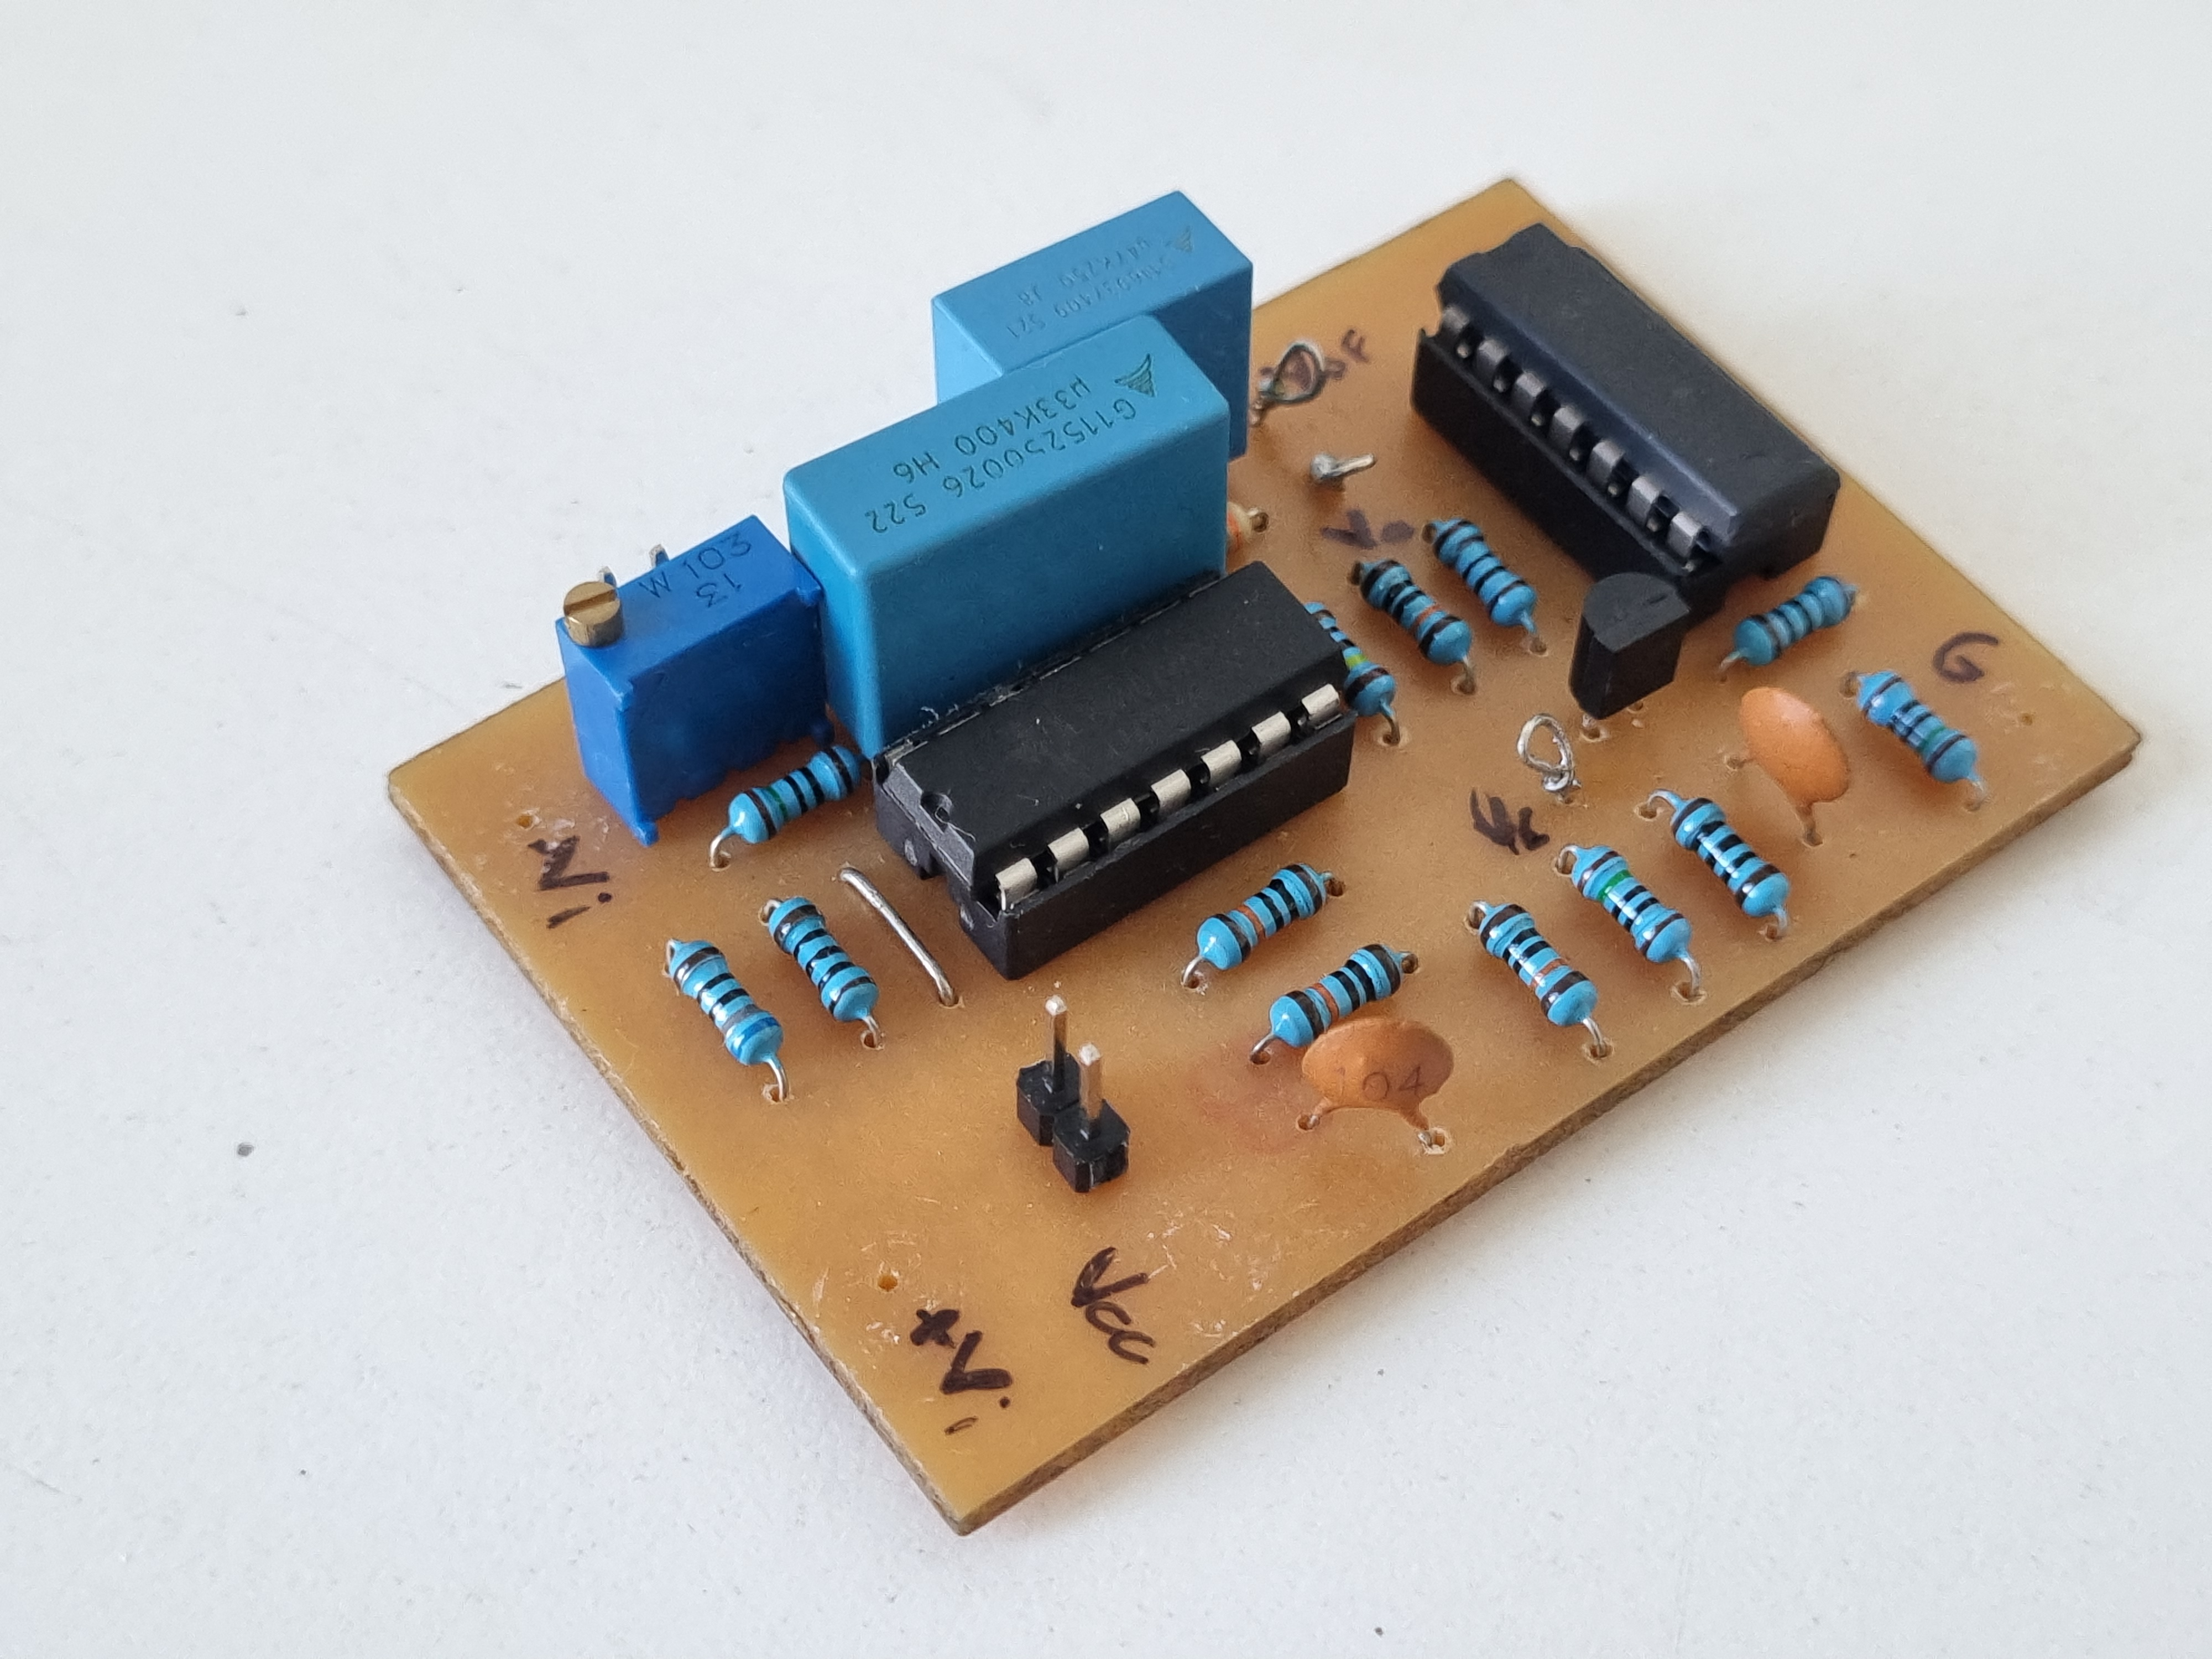
\includegraphics[width=0.70\textwidth]{pcb_lazo_4-20ma.jpg}
\caption{Placa de circuito impreso implementada para el acondicionador de señal de campo de $4\text{--}20\,\mathrm{mA}$.}
\label{fig.ej1:placa}
\end{figure}

\section{Mediciones de Laboratorio y Resolución del Problema de Polarización}
\label{sec.ej1:mediciones}

Una vez montado el circuito completo en placa de circuito impreso (Figura~\ref{fig.ej1:placa}), se procedió a la
etapa de medición y verificación experimental.

\subsection{Detección del Problema en el Amplificador de Instrumentación}
Al iniciar los ensayos inyectando una corriente de entrada de fondo de escala ($I_{\text{in}} = 20 \unit{\milli\ampere}$),
con una caída en el *shunt* de $V_{\text{diff}} = 5.00 \unit{\volt}$, se observó una discrepancia considerable: la
tensión a la salida del restador y del filtro alcanzaba únicamente $4.50 \unit{\volt}$, registrando una pérdida neta
de aproximadamente $500 \unit{\milli\volt}$ respecto al valor nominal esperado.

Al contrastar este comportamiento con la hoja de datos del fabricante del LM324 y con la simulación del punto de
operación en continua (\texttt{ampli\_instrumentacion\_op.txt}), identificamos la causa física:
\begin{enumerate}
    \item El seguidor $U_{1A}$ toma el borne negativo del lazo referenciado a masa mediante $R_{\text{CM}} = 1 \unit{\mega\ohm}$,
    por lo que su salida debe aproximarse a $0 \unit{\volt}$ (condición de cierre a masa).
    \item Con la entrada diferencial en $5 \unit{\volt}$, el seguidor $U_{1B}$ se sitúa en $5 \unit{\volt}$. El divisor
    $R_4\text{--}R_5$ fija la entrada no inversora del restador $U_{1C}$ en $2.50 \unit{\volt}$, trasladándose por
    cortocircuito virtual a su entrada inversora ($V_- = 2.50 \unit{\volt}$).
    \item Con las resistencias de $10 \unit{\kilo\ohm}$ propuestas originalmente por la consigna, la resistencia $R_3$
    vincula directamente el nodo $V_- = 2.50 \unit{\volt}$ con la salida de $U_{1A}$ ($V_{o,U1A} \approx 0 \unit{\volt}$),
    exigiendo a la etapa de salida de $U_{1A}$ drenar hacia masa una corriente de sumidero (*current sink*) de:
    \begin{equation}
    \label{eq.ej1:isink_falla}
    I_{\text{sink}} = \frac{2.50 \unit{\volt} - 0 \unit{\volt}}{10 \unit{\kilo\ohm}} = 250 \unit{\micro\ampere}
    \end{equation}
    En la simulación SPICE de punto de operación, la corriente registrada en $R_3$ alcanzó $I(R_3) = 309 \unit{\micro\ampere}$
    debido a las tensiones efectivas de modo común.
    \item Según la hoja de datos del LM324, para tensiones de salida muy próximas a masa ($V_o \le 200 \unit{\milli\volt}$),
    la capacidad de sumidero está limitada por una fuente interna de corriente constante de solo $50 \unit{\micro\ampere}$
    típicos ($12 \unit{\micro\ampere}$ mínimos). Al ser sobrepasada por los $250\text{--}309 \unit{\micro\ampere}$, la
    salida no puede bajar a masa y se eleva a la tensión necesaria para encender el transistor NPN inferior de la etapa
    push-pull ($V_{\text{CE,sat}} + V_{\gamma} \approx 500 \unit{\milli\volt}$).
    \item Esta elevación de $500 \unit{\milli\volt}$ en la referencia de masa del restador provocó directamente que
    la salida entregara $V_{E1} = 5.00 \unit{\volt} - 0.50 \unit{\volt} = 4.50 \unit{\volt}$.
\end{enumerate}

Para resolver el problema, reemplazamos las cuatro resistencias del restador ($R_3, R_4, R_5, R_f$)
de $10 \unit{\kilo\ohm}$ por resistores de $100 \unit{\kilo\ohm}$. Con ello, la corriente exigida se redujo a:
\begin{equation}
\label{eq.ej1:isink_ok}
I_{\text{sink}} = \frac{2.50 \unit{\volt}}{100 \unit{\kilo\ohm}} = 25 \unit{\micro\ampere}
\end{equation}

Como $25 \unit{\micro\ampere} < 50 \unit{\micro\ampere}$, la corriente quedó dentro de la capacidad del integrado,
la salida del seguidor descendió a $2.64 \unit{\milli\volt}$ (corroborado en simulación SPICE) y el problema quedó
completamente solucionado, obteniendo la respuesta lineal esperada.

\subsection{Caracterización Estática}
Tras la modificación, se inyectaron corrientes de prueba de $4 \unit{\milli\ampere}$ a $20 \unit{\milli\ampere}$,
registrando simultáneamente las tensiones y la corriente de salida hacia el PLC (Tabla~\ref{tab.ej1:estatica}).

\begin{table}[!ht]
\centering
\small
\begin{tabular}{ccccc}
\toprule
$I_{\text{in}}$ [$\unit{\milli\ampere}$] & $V_{\text{diff}}$ ($E_1$) [$\unit{\volt}$] & $V_{\text{filtro}}$ ($E_2$) [$\unit{\volt}$] & $I_{\text{out}}$ ($E_3$) [$\unit{\milli\ampere}$] & Error relativo \\
\midrule
$4.00$  & $1.002$ & $1.001$ & $3.98$  & $-0.50\%$ \\
$8.00$  & $2.005$ & $2.004$ & $7.96$  & $-0.50\%$ \\
$12.00$ & $3.010$ & $3.008$ & $11.93$ & $-0.58\%$ \\
$16.00$ & $4.012$ & $4.010$ & $15.91$ & $-0.56\%$ \\
$20.00$ & $5.018$ & $5.015$ & $19.89$ & $-0.55\%$ \\
\bottomrule
\end{tabular}
\caption{Caracterización estática de linealidad del sistema tras el cambio a $100\,\mathrm{k}\Omega$.}
\label{tab.ej1:estatica}
\end{table}

\subsection{Caracterización Dinámica y Atenuación a 50 Hz}
Se inyectó una señal senoidal de $V_i = 4.521 \unit{\volt}_{\text{pp}}$ con offset de continua y se barrieron
frecuencias desde $1 \unit{\hertz}$ hasta $70 \unit{\hertz}$ (Tabla~\ref{tab.ej1:dinamica}).

\begin{table}[!ht]
\centering
\small
\begin{tabular}{ccccc}
\toprule
$f$ [$\unit{\hertz}$] & $V_i$ [$\unit{\volt}$] & $V_o$ [$\unit{\volt}$] & $V_o/V_i$ [$\unit{\volt\per\volt}$] & Atenuación [$\unit{\decibel}$] \\
\midrule
$1.0$  & $4.521$ & $4.521$ & $1.000$ & $0.00 \unit{\decibel}$ \\
$2.0$  & $4.521$ & $4.521$ & $1.000$ & $0.00 \unit{\decibel}$ \\
$3.0$  & $4.521$ & $4.441$ & $0.982$ & $-0.15 \unit{\decibel}$ \\
$4.0$  & $4.521$ & $4.321$ & $0.956$ & $-0.39 \unit{\decibel}$ \\
$5.0$  & $4.521$ & $4.201$ & $0.929$ & $-0.64 \unit{\decibel}$ \\
$6.0$  & $4.521$ & $4.081$ & $0.903$ & $-0.89 \unit{\decibel}$ \\
$7.0$  & $4.521$ & $3.921$ & $0.867$ & $-1.24 \unit{\decibel}$ \\
$8.0$  & $4.521$ & $3.681$ & $0.814$ & $-1.79 \unit{\decibel}$ \\
$9.0$  & $4.521$ & $3.481$ & $0.770$ & $-2.27 \unit{\decibel}$ \\
$10.0$ & $4.521$ & $3.241$ & $0.717$ & $-2.89 \unit{\decibel}$ \\
$14.5$ & $4.521$ & $2.241$ & $0.496$ & $-6.09 \unit{\decibel}$ \\
$20.0$ & $4.521$ & $1.425$ & $0.315$ & $-10.03 \unit{\decibel}$ \\
$30.0$ & $4.521$ & $0.750$ & $0.166$ & $-15.60 \unit{\decibel}$ \\
$40.0$ & $4.521$ & $0.480$ & $0.106$ & $-19.48 \unit{\decibel}$ \\
$50.0$ & $4.521$ & $0.300$ & $0.066$ & $-23.56 \unit{\decibel}$ \\
$60.0$ & $4.521$ & $0.200$ & $0.044$ & $-27.08 \unit{\decibel}$ \\
$70.0$ & $4.521$ & $0.150$ & $0.033$ & $-29.58 \unit{\decibel}$ \\
\bottomrule
\end{tabular}
\caption{Respuesta en frecuencia experimental del filtro activo de campo.}
\label{tab.ej1:dinamica}
\end{table}

A $10.0 \unit{\hertz}$ la tensión cayó a $3.241 \unit{\volt}$ ($-2.89 \unit{\decibel}$), validando la frecuencia de
corte nominal de diseño. A la frecuencia de interferencia de $50.0 \unit{\hertz}$, la amplitud descendió a
$0.300 \unit{\volt}$, representando una atenuación de $-23.56 \unit{\decibel}$.

\subsection{Registro Osciloscópico}
Las Figuras~\ref{fig.ej1:osc_2hz} y~\ref{fig.ej1:osc_50hz} presentan las mediciones en el dominio temporal:

\begin{figure}[!ht]
\centering
\begin{subfigure}[t]{0.48\textwidth}
    \centering
    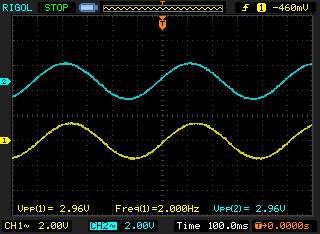
\includegraphics[width=\textwidth]{lazo_osc_2hz.png}
    \caption{Entrada (amarillo) y salida (cian) a $2\,\mathrm{Hz}$: $V_{\text{pp}} = 2.96\,\mathrm{V}$ en ambos canales (ganancia unitaria).}
    \label{fig.ej1:osc_2hz}
\end{subfigure}
\hfill
\begin{subfigure}[t]{0.48\textwidth}
    \centering
    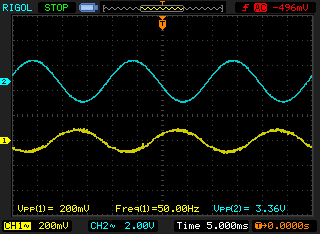
\includegraphics[width=\textwidth]{lazo_osc_50hz.png}
    \caption{Atenuación a $50\,\mathrm{Hz}$: entrada senoidal de $3.36\,\mathrm{V}_{\text{pp}}$ reducida a $200\,\mathrm{mV}_{\text{pp}}$ ($-24.5\,\mathrm{dB}$).}
    \label{fig.ej1:osc_50hz}
\end{subfigure}
\caption{Formas de onda en el osciloscopio para el sistema acondicionador de campo.}
\label{fig.ej1:tiempo}
\end{figure}

\begin{figure}[!ht]
\centering
\begin{subfigure}[t]{0.48\textwidth}
    \centering
    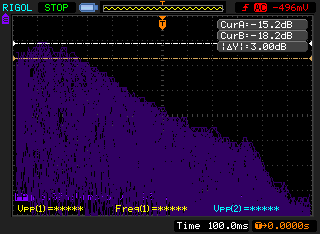
\includegraphics[width=\textwidth]{lazo_fft_mag.png}
    \caption{Perfil espectral FFT: cursores ajustados a $\Delta Y = 3.00\,\mathrm{dB}$ ($CurA = -15.2\,\mathrm{dB}$, $CurB = -18.2\,\mathrm{dB}$).}
    \label{fig.ej1:fft_mag}
\end{subfigure}
\hfill
\begin{subfigure}[t]{0.48\textwidth}
    \centering
    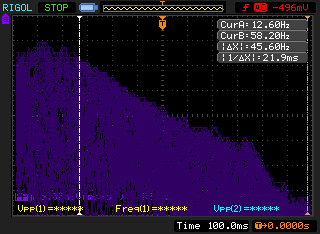
\includegraphics[width=\textwidth]{lazo_fft_fc.png}
    \caption{Medición de $f_c$ a $-3\,\mathrm{dB}$ mediante FFT: $CurA = 12.60\,\mathrm{Hz}$.}
    \label{fig.ej1:fft_fc}
\end{subfigure}
\caption{Análisis por transformada rápida de Fourier (FFT) del filtro en osciloscopio digital.}
\label{fig.ej1:fft}
\end{figure}

Mediante el análisis FFT del osciloscopio (Figura~\ref{fig.ej1:fft}), la frecuencia de corte real a $-3 \unit{\decibel}$
se situó en $f_c = 12.60 \unit{\hertz}$, compatible con las tolerancias de los capacitores comerciales de poliéster.
